\documentclass[]{article}
\usepackage{graphicx}
\usepackage{amsmath}
%opening
\title{Nociones Básicas de programación C}
\author{Antonio Torres}

\begin{document}

\maketitle

\begin{abstract}
En este documento se abordan las nociones básicas de los lenguajes de programación en general, desde el proceso de escritura del programa hasta su salida. Se habla acerca de la historia del lenguaje C, los tipos de datos que lo conforman y sus características.
\end{abstract}

\tableofcontents

\pagebreak
\section{Compiladores}
El compilador es un programa con el propósito de traducir el código fuente a lenguaje máquina, este programa tomará como datos nuestro programa escrito en lenguaje de alto nivel y dará como salida el mismo programa pero escrito en lenguaje maquina, este mismo ya puede ser ejecutado de manera directa o indirecta en el ordenador.
% TODO: \usepackage{graphicx} required
\begin{figure}[h!]
	\centering
	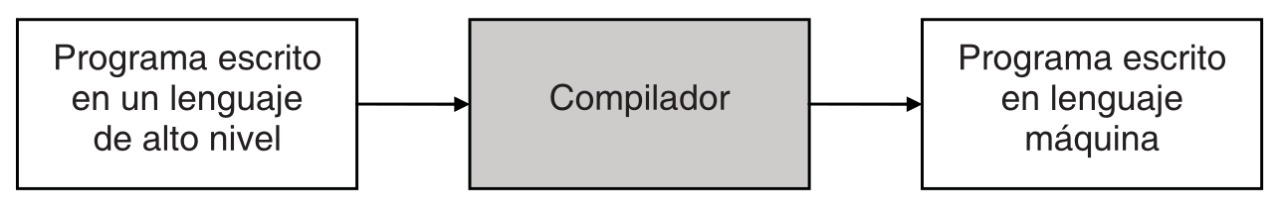
\includegraphics[width=0.7\linewidth]{"img/proceso de compilacion.jpeg"}
	\caption{Proceso de compilación}
	\label{fig:proceso-de-compilacion}
\end{figure}

Por ejemplo, un programa escrito en en lenguaje C necesita un compilador especial para el lenguaje C para poder ser traducido. Posteriormente, el programa traducido podrá ser ejecutado de manera directa por el ordenador. 

\section{Intérpretes}
A diferencia de un compilador, un interprete no genera un programa escrito en lenguaje maquina a partir del código fuente, sino que efectúa la traducción y ejecución de manera simultanea para cada una de las sentencias e instrucciones del programa. Por ejemplo, un programa escrito en Python necesita del intérprete de Python para ser ejecutado. Durante el proceso de ejecución de cada una de las sentencias del programa ocurre de manera simultanea su traducción.

A diferencia de un compilador el interprete hace que la ejecución de un programa resulte ser mas lenta, debido a que el interprete acarrea una traducción simultanea.

\section[Ventajas y desventajas]{El lenguaje C}
C es un lenguaje de programación de alto nivel con el que se pueden escribir programas con fines muy diversos. Originalmente fue desarrollado por Dennis Ritchie entre 1969 y 1972 en los laboratorios Bell de AT\&T, como una evolución del lenguaje de programación B.

Al igual que el lenguaje B, C está orientado a la implementación de sistemas operativos, concretamente en sistemas tipo UNIX. En 1972, Dennis Ritchie toma revelo y modifica el lenguaje B, creando el lenguaje de programación C y reescribiendo UNIX en dicho lenguaje. La novedad que introdujo el lenguaje C sobre B fue el diseño de tipos y estructuras de datos, entre ellas: \textbf{char, int, float, double, short (enteros con longitud $\leq$ a int), long (enteros de longitud $\geq$ a int), unsigned (enteros sin signo) y enumeraciones.}

Los tipos estructurados básicos de C son las \textbf{estructuras, uniones y matrices.} A partir de los tipos básicos es posible definir tipos derivados de mayor complejidad.

Una de las ventajas significativas de C sobre los de más lenguajes de programación es que el codigo generado por el compilador C está muy optimizado en tamaño, lo que redunda en una mayor velocidad en ejecución. Algunas de las bondades de C son las siguientes: 
\begin{itemize}
	\item Programación estructurada.
	\item Abundancia en operadores y tipos de datos.
	\item Reemplaza ventajosamente la programación en ensamblador.
	\item Codificación en bajo y alto nivel simultáneamente.
	\item Facilidad de aprendizaje.
	\item Soporte a recursividad.
\end{itemize}

\section{Tipos de datos en C}
Los tipos de datos en C se clasifican en primitivos y derivados.
\subsection{Tipos de datos primitivos}
A este tipo de datos se les llama primitivos porque estan definidos por el compilador. Hay siete tipos de datos primitivos que podemos clasificar en tipos enteros y reales.

\begin{itemize}
	\item \textbf{Tipos enteros: } char, short, int, long y enum.
	\item \textbf{Tipos reales: } float y double.
\end{itemize}

Cada tipo primitivo tiene un rango diferente de los valores positivos y negativos. El tipo de datos seleccionado para declarar las variables de un determinado programa dependerá del rango y tipo de valores que vayan a almacenar cada una de ellas y de si estos son enteros o fraccionarios. Los ficheros de cabecera \textbf{limits.h} y \textbf{float.h} especifican los valores máximo y mínimo para cada tipo.

Cada tipo de entero puede ser calificado por las palabras \textbf{signed} o \textbf{unsigned}. Un entero clasificado como signed es un entero con signo; esto es, un valor entero positivo o negativo. Un entero clasificado como unsigned es un valor entero sin signo, el cual es manipulado como un valor entero positivo. Estas clasificaciones dan lugar a los siguientes tipos extras: 

\begin{itemize}
	\item unsigned char, signed char
	\item unsigned short, signed short
	\item unsigned int, signed int
	\item unsigned long, signed long
\end{itemize}

Si los calificadores signed y unsigned se utilizan sin un tipo entero especifico, se asume el tipo int, por lo tanto:

\begin{itemize}
	\item \textbf{signed x;} es equivalente a \textbf{signed int x;}
\end{itemize}

\subsubsection{char}
El tipo de dato char o caracter se usa para declarar datos comprendidos entre $-128$ y $+127$. Podemos definir los char como un conjunto de ocho bits, de los cuales uno de ellos es para especificar el signo y el resto para el valor; dicho conjunto de bits recibe el nombre de byte.
El tipo \textbf{unsigned char} puede almacenar valores en el rango de 0 a 255, ya que ahora no es necesario emplear un bit para el signo. Los valores comprendidos de 0 a 127 corresponden con los 128 primeros caracteres del los códigos internacionales ASCII, ANSI o UNICODE empleados para la representación de caracteres.

\subsubsection{short}
el tipo short, abreviatura de \textbf{signed short int}, se usa para declarar datos enteros correspondidos entre -32738 y 32738. En tipo short se define como un dato de 16 bits de longitud.

\subsubsection{int}
Los tipos de datos int, abreviatura de \textbf{signed int} comprende valores desde -2147483648 y -2147483648. Un valor int se define como un dato de 32 bits de longitud.
El tipo \textbf{unsigned int} puede almacenar valores en el rango de 0 a 4294967295 ya que ahora no es necesario usar un bit para el signo.

\subsubsection{long}
El tipo de dato long se usa para declarar valores enteros comprendidos entre -2147483648 y +2147483648. Un valor tipo long se define como un dato de 32 bits de longitud (en otros compiladores es de 64 bits).

\subsubsection{enum}
La declaración tipo enum es una lista de valores que pueden ser tomados por una variable de ese tipo. Los valores de un tipo enumerado se representaran con identificadores, que seran constantes del nuevo tipo.
\begin{figure}[h!]
	\centering
	\includegraphics[width=0.7\linewidth]{"img/enum"}
	\caption{Ejemplo declaración de una enumeración.}
	\label{fig:proceso-de-compilacion}
\end{figure}

donde tipo\_enumerado es un identificador que nombra en nuevo tipo definido.

\subsubsection{float}
El tipo de dato float se usa para declarar un dato en coma flotante de 32 bits en el formato IEEE 754. Los datos tipo float almacenan valores con una precisión aproximada de los siete dígitos.

\subsubsection{double}
El tipo double se usa para almacenar un dato coma flotante de 64 bits en el formato IEEE 754. Los datos tipo double almacenan valores con una precisión aproximada de 16 dígitos.

\subsection{Tipos de datos derivados}
Los tipos derivados son construidos a partir de los tipos de datos primitivos. Algunos de ellos son: \textbf{estructuras, uniones, matrices, punteros y funciones.}

\subsection{Sinonimos de un tipo}
Usando la palabra reservada \textbf{typedef} podemos declarar nuevos nombres de tipos de datos, o mejor dicho sinónimos o alias de otro tipo de dato, ya sea primitivo o derivado, los cuales pueden ser usados más tarde para declarar variables de esos tipos.

Las declaraciones \textbf{typedef} permiten parametrizar un programa para evitar problemas de portabilidad. Si usamos sinonimos de tipos de datos con typedef los tipos que pueden depender de la instalacion, cuando se lleve el programa a otra instalacion solo se tendrán que cambiar estas declaraciones.

\subsection{Palabras reservadas}
Las palabras reservadas son identificadores predeterminados que tienen un significado especial para el compilador de C. Por lo tanto, un identificador definido por el usuario no puede tener el mismo nombre que una palabra reservada.

\pagebreak
\section{Operadores}
\subsection{Operadores a nivel de bits}
Este tipo de operadores permiten realizar con sus operandos las operaciones AND, OR, XOR y desplazamientos, bit por bit. Los operadores tienen que ser enteros.
\begin{align}
	\begin{tabular}{|c|c|}
		\hline
		\& & Operacion AND a nivel de bits \\
		\hline
		| & Operacion OR a nivel de bits (caracter ASCII 128) \\
		\hline
		\^{}z| & Operacion XOR a nivel de bits \\
		\hline
		<< & Desplazamiento a la izquierda rellenando con ceros por la derecha \\
		\hline
		>> & Desplazamiento a la derecha rellenando con el bit de signo por la izquierda \\
		\hline
	\end{tabular}
\end{align}

\subsection{Operación dirección de}
El operador \& (dirección en memoria de) nos permite obtener la dirección en memoria de su operando.

\subsection{Operador de in-dirección}
El operador de indireccion *(indirección) accede a un valor indirectamente a través de una dirección (un puntero). El resultado es el valor direccionado por el operando; dicho de una manera mas sencilla, el valor apuntado por el puntero.

Un \textbf{puntero} es una variable con la capacidad de almacenar una direccion de memoria que indica donde se localiza un dato de un tipo especificado. La sintáxis para definir un puntero es la siguiente:

\begin{align}
	\textit{tipo * identificador}
\end{align}

donde tipo es el tipo de dato apuntado, ya sea primitivo o derivado

\end{document}
